\chapter{Threats of Blockchain}
The Blockchain \cite{blockchainAttacks} is a technology used in various applications, such as cryptocurrencies, Internet of Things, electronic voting and many others. Its transparent, fully distributed, peer to peer and append-only nature are its most notable strengths. The transactions, which may have a different meaning depending on the application they are used for, are publicly visible and cannot be modified after they are published. This means the users may verify any transaction with no need of a centralized authority.

Bitcoin, the most popular cryptocurrency at this moment, takes advantage of these characteristics, creating a decentralized financial system. Unfortunately, there are also significant shortcomings in terms of security. One of the most notorious instances where these vulnerabilities had been exploited is known as ``The DAO'' \cite{blockchainAttacks}, where in 2016, an unknown attacker managed to drain \$50 million USD through a \textit{Reentrancy Attack}.

This thesis will first present the variety of attacks that blockchain networks are vulnerable to, their manner of work and potential effects to its victims. The Quadriga Initiative \cite{quadriga}  - a community-based platform - hosts a list of most of the attacks and frauds that involve cryptocurrency exchanges. Among the most well-known attacks, the database of case studies includes instances of Reentrancy Attacks, Replay Attacks and Short Address Attacks.

\textit{Reentrancy Attacks} \cite{reentrancy} can take place whenever the developers of the targeted network do not update the balances before sending the funds. In this case, an attacker could recursively call the withdraw() method and drain all the available funds. 

\textit{Replay Attacks} \cite{replay} are specific to the case where a cryptocurrency is forked into two separate currencies. In such a scenario, it is possible to sniff a regular transaction from any of the chains and “replay” it on the other. Processing both transaction causes the user to lose the same amount of assets twice (for example, paying two ether instead of one for the same product or service). This attack was easily possible in the Ethereum blockchain before the implementation of chainID in transactions.

\textit{Short Address Attacks} \cite{blockchainAttacks} represent the exploit of a bug in the EVM – Ethereum Virtual Machine – used to obtain extra tokens on purchases. This category of attacks requires creating an Ethereum wallet with its address ending with a 0 byte. The attacker makes a purchase on the address by removing the last digit and causes the contract to try to append the missing byte to the incomplete address, but it ends up appending it to the paid amount. In this case, the contract pays 256 times more tokens than intended. 

In terms of prevention and detection of such attacks, there are numerous tools that serve this purpose. As Kaixuan Li et al. describe in their article \cite{staticAnalysisToolsComparison}, a significant category of such tools detect vulnerabilities in the code through either static analysis or symbolic execution.


\begin{table}[h]
\centering
\begin{tabular}{cccc}
\hline
Technology         & Tool       & Analysis Level & Stars \\ \hline
                   & Securify2  &                & 529   \\
Static Analysis    & Slither    & Source Code    & 4 500 \\
                   & SmartCheck &                & 315   \\ \hline
                   & Manticore  &                & 3 500 \\
Symbolic Execution & Osiris     & Bytecode       & 50    \\
                   & Oyente     &                & 1 300 \\ \hline
\end{tabular}
\caption{List of the main static analysis and symbolic execution tools, adapted from Kaixuan Li et al. \cite{staticAnalysisToolsComparison}}
\end{table}

According to table 1.1, the static analysis tools, primarly represented by Slither, enjoy a higher popularity than the symbolic execution tools, represented by Manticore. This fact is shown by the number of stars on GitHub, which indicate how popular a tool is. These types of tools share the principle of scanning the code without executing it, but do so in different ways.

Generally, static analysis tools \cite{staticAnalysisDef} are automatic methods that determine the run-time properties of a program without running it. In Slither's \cite{slither} case, the analysis' purpose is to detect security vulnerabilities within the smart contract and to point out potential optimizations, which result in a lower gas consumption, an essential aspect in this field. As such, this category of security tools should be considered the opposite of Dynamic Analysis tools, which rely on running the target program and can also monitor it's performance among other aspects.

On the other hand, symbolic execution tools \cite{symbolicExecutionDef} take a similar approach of analyzing the given program without running the code, based solely on its bytecode. Esentially, Manticore \cite{manticore} uses the bytecode of a smart contract to map out all the execution paths of the program. Afterwards, all the paths get explored and the tool determines what kind of inputs determine each possible outcome. Two of the main components of Manticore are the Core Engine and the Event System. The Core Engine is responsible with operating and managing the state of a program at a certain point in the execution. The Execution Module has the purpose to emulate a system that runs the target program, with a CPU, system memory and an operating system like Linux.

\begin{figure}[H]
\centering
\begin{BVerbatim}
int foobar(int a, int b) {
    int x = 1, y = 0;
    if (a != 0) {
        y = 3 + x;
        if (b == 0) {
            x = 2 * (a + b);
        }
    }
    assert(x - y != 0);
}
\end{BVerbatim}
\caption{Example of code to analyze. From Roberto B et al. \cite{symbolicExecutionDef}}
\end{figure}

The figure above shows a simple example of function that a symbolic execution tool can operate on. A tool like Manticore can trace all the possible paths the execution may go at run-time. The assertion at the end is the possible point of failure for this function, in case \texttt{x} and \texttt{y} are equal.

\begin{figure}[H]
\centering
\resizebox{\textwidth}{!}{%
\usetikzlibrary{arrows.meta}

\begin{tikzpicture}[
  node distance=0.8cm and 1.6cm,
  every node/.style={font=\small},
  box/.style={rectangle, draw, rounded corners, align=left, text width=7cm, minimum height=1.2cm},
  ok/.style={ellipse, draw, align=center, minimum height=1cm, minimum width=2cm},
  error/.style={ellipse, draw=red, text=red, align=center, minimum height=1cm, minimum width=3.5cm},
  ->, >=Stealth
]

% Nodes
\node[box] (A) {\textbf{A}\\$\sigma = \{a \mapsto \alpha_a, b \mapsto \alpha_b\}$\\$\pi = \text{true}$\\2. int x = 1, y = 0};

\node[box, below=of A] (B) {\textbf{B}\\$\sigma = \{a \mapsto \alpha_a, b \mapsto \alpha_b, x \mapsto 1, y \mapsto 0\}$\\$\pi = \text{true}$\\3. if (a != 0)};

\node[box, below left=of B] (C) {\textbf{C}\\$\sigma = \{a \mapsto \alpha_a, b \mapsto \alpha_b, x \mapsto 1, y \mapsto 0\}$\\$\pi = \alpha_a \neq 0$\\4. y = 3 + x};

\node[box, below=of C] (E) {\textbf{E}\\$\sigma = \{a \mapsto \alpha_a, b \mapsto \alpha_b, x \mapsto 1, y \mapsto 4\}$\\$\pi = \alpha_a \neq 0$\\5. if (b == 0)};

\node[box, below=of E] (F) {\textbf{F}\\$\sigma = \{a \mapsto \alpha_a, b \mapsto \alpha_b, x \mapsto 1, y \mapsto 4\}$\\$\pi = \alpha_a \neq 0 \land \alpha_b = 0$\\6. x = 2 * (a + b)};

\node[box, below=of F] (H) {\textbf{H}\\$\sigma = \{a \mapsto \alpha_a, b \mapsto \alpha_b, x \mapsto 2(\alpha_a + \alpha_b), y \mapsto 4\}$\\$\pi = \alpha_a \neq 0 \land \alpha_b = 0$\\8. assert(x - y != 0)};

\node[error, below=of H] (ERR) {ERROR\\$2(\alpha_a + \alpha_b) - 4 = 0 \land \alpha_a \neq 0 \land \alpha_b = 0$ \\\\ $\text{if } \alpha_a = 2 \land \alpha_b = 0$};

\node[box, below right=of E] (G) {\textbf{G}\\$\sigma = \{a \mapsto \alpha_a, b \mapsto \alpha_b, x \mapsto 1, y \mapsto 4\}$\\$\pi = \alpha_a \neq 0 \land \alpha_b \neq 0$\\8. assert(x - y != 0)};

\node[ok, below=of G] (OKG) {OK\\$1 - 4 = 0 \land \alpha_a \neq 0 \land \alpha_b \neq 0 \Leftrightarrow \text{false}$};

\node[box, below right=of B] (D) {\textbf{D}\\$\sigma = \{a \mapsto \alpha_a, b \mapsto \alpha_b, x \mapsto 1, y \mapsto 0\}$\\$\pi = \alpha_a = 0$\\8. assert(x - y != 0)};

\node[ok, below=of D] (OKD) {OK\\$1 - 0 = 0 \land \alpha_a = 0 \Leftrightarrow \text{false}$};

% Edges
\draw[->] (A) -- (B);
\draw[->] (B) -- node[left] {$\alpha_a \neq 0$} (C);
\draw[->] (B) -- node[right] {$\alpha_a = 0$} (D);
\draw[->] (C) -- (E);
\draw[->] (E) -- node[left] {$\alpha_b = 0$} (F);
\draw[->] (E) -- node[right] {$\alpha_b \neq 0$} (G);
\draw[->] (F) -- (H);
\draw[->] (H) -- (ERR);
\draw[->] (G) -- (OKG);
\draw[->] (D) -- (OKD);

\end{tikzpicture}%
}
\caption{Example of symbolic execution tree of function \texttt{foobar}. Each state shows the symbolic store $\sigma$, the path constraint $\pi$, and the current statement. From Roberto B. et al \cite{symbolicExecutionDef}}
\end{figure}

As shown in this graph, $\sigma$ contains all the symbols stored in the context of the function, $\pi$ is a statement that represents the path constraint and below it is the line of code that gets excecuted at a given time. State \textit{B} is the first one to fork in two hypothetical states, based on the value of the first parameter, as shown by $\pi$ in the states \textit{C} and \texttt{D}. If \texttt{a == 0}, the function skips to the final assert and returns with no failure. Otherwise, the program would continue with state \texttt{E} and the following ones. Finally, a symbolic execution tool can reveal that the function will throw an error in case \texttt{a == 2 and b == 0}.

\begin{table}
\centering
\begin{tabular}{ccccl}
\hline
\multirow{2}{*}{Tool} & \multirow{2}{*}{\# Success} & \multicolumn{3}{c}{\# Failure}         \\ \cline{3-5} 
                      &                             & \# Timeout & \# Compilation & \# Total \\ \hline
Slither               & 767 (97.34\%)               & 2          & 19             & 21       \\
Manticore             & 112 (14.21\%)               & 626        & 50             & 676      \\ \hline
\end{tabular}
\caption{Success rate and failures summary of Slither and Manticore. Adapted from Kaixuan Li et al. \cite{staticAnalysisToolsComparison}}
\label{tab:my-table2}
\end{table}

Finally, to address Manticore's performance, as shown above, its exhaustive approach causes it to fail most of the tests due to timeout. Even if we were to ignore the timeout fails, Slither is visibly more consistent, having less compilation failures. The main flaw and reason of Manticore's high timeout rate may be the fact that it has to process large amounts of possible paths in order to find the ones where a security flaw is exploited. As such, Slither is the more consistent and better performing in comparison to Manticore.

\section{Slither}

Considering the performance metrics discussed in the first section, this section will be dedicated to Slither \cite{slither}, a static analysis tool catered to smart contracts written in Solidity and designed to offer granular information about smart contract code. This tool specializes in vulnerability detection, but also manages to point out potential optimizations that lower the gas consumption of a smart contract. In order to facilitate the usage of this tool, Slither leverages printers to help the user better understand the contract’s functionality and structure. This is done through representations such as the control flow graph or the inheritance graph or summaries of the contract and the issues detected in its code. 

In opposition to dynamic analysis \cite{dynamicAnalysis} tools, which rely on executing the contract’s code to find security weaknesses, static analysis tools detect vulnerabilities without running the smart contract. Such approaches include parsing and decompiling the EVM bytecode and translating it into semantic facts. These semantic facts are then matched with predefined patterns meant to reveal common issues.

Slither \cite{slither} proceeds in a similar manner by taking the Solidity Abstract Syntax Tree generated by the compiler and extracting information such as the control flow graph and transforms the code given into SlithIR, its internal representation language. After these two initialization stages, the actual code analysis takes place. In this stage, Slither identifies the reads and writes of variables, analyses the data dependency and determines whether the methods are protected from unauthorized use (for instance, only the owner of a contract may create new tokens).

This tool \cite{slither} helps auditors detect various vulnerabilities and potential security threats, such as reentrancy attacks or uninitialized storage variables. Its aproach of quickly transalating and analyzing large codebases makes it significantly faster than symbolic execution engines, as shown Table 1.2, a great feature for fast development workflows.

Furthermore, its set of detectors are able to find obvious and subtle vulnerabilities alike while providing useful educational resources to help developers fix and prevent future attacks. All these factors make Slither a great solution for quick and automated daily audit processes, preventing many critical security vulnerabilities.

Another essential topic in blockchain development, beside security concerns, is optimization, the techniques used to lower the ``gas'' consumption. Slither includes a set of detectors specialized in finding ways to optimize code \cite{slitherGitHub} from different perspectives. They are able to find issues such as dead code, as in methods or code branches that are never called or executed, unused state variables or variables that should be declared constant to save gas.

\begin{figure}[h]
    \centering
    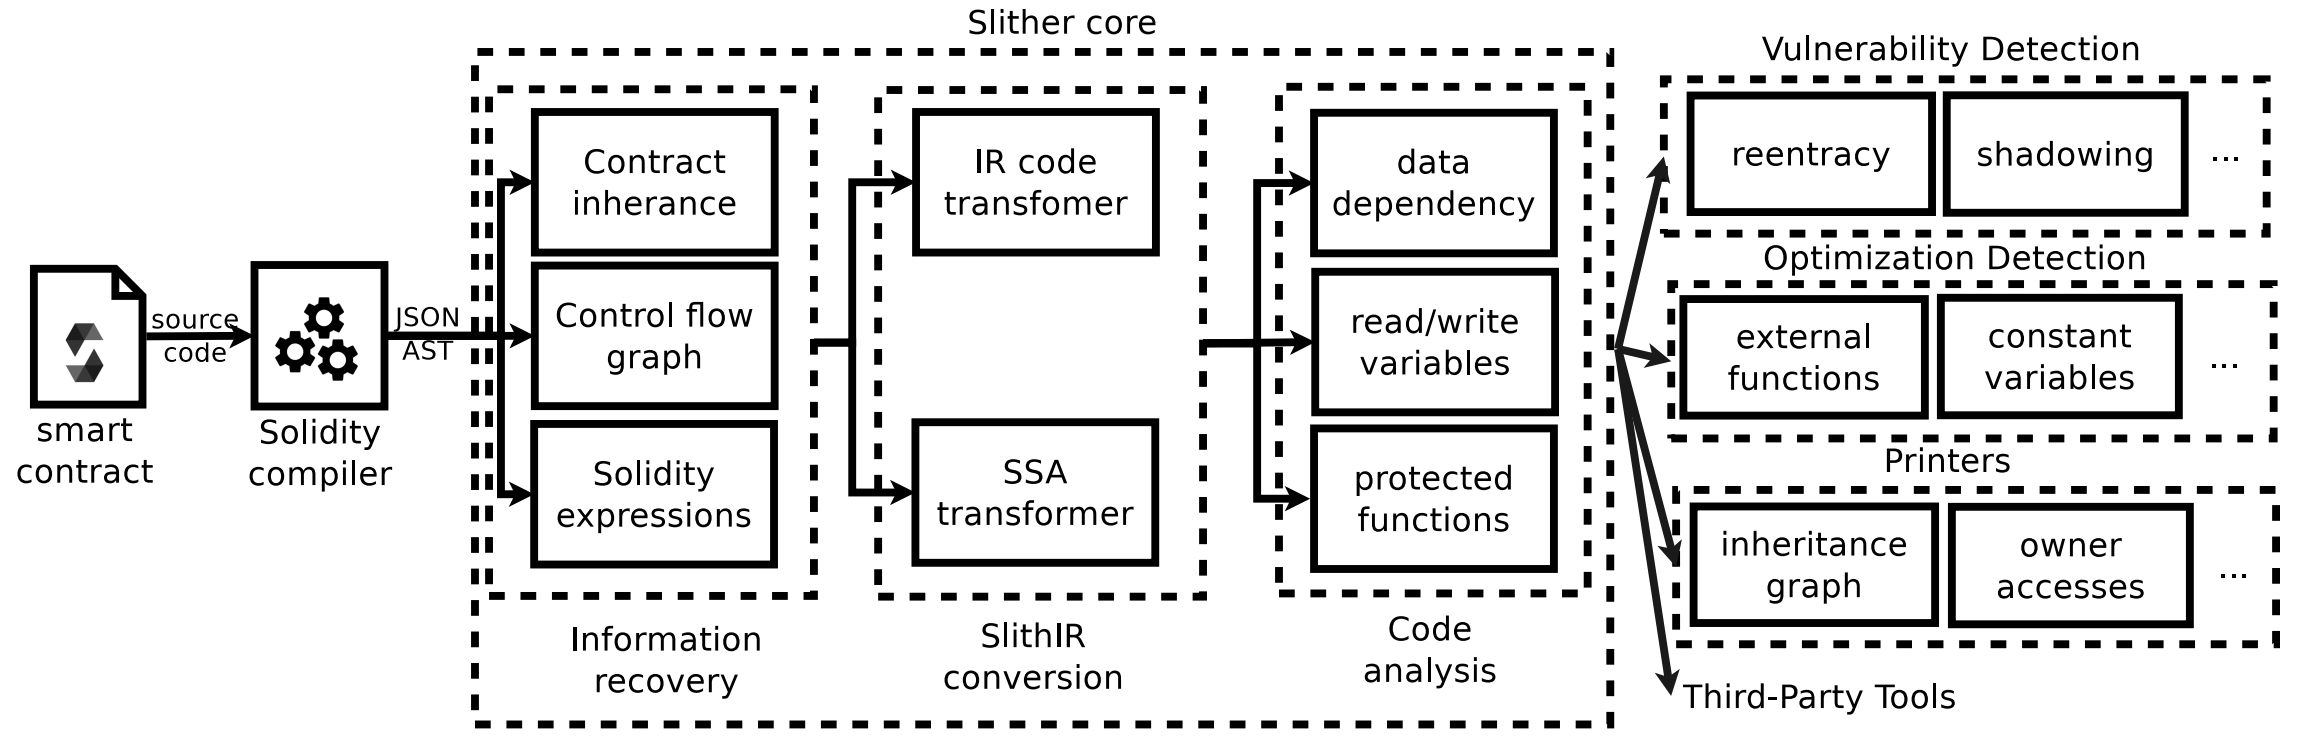
\includegraphics[width=1\linewidth]{images/image.png}
    \caption{Slither overview. From Josselin F. et al. \cite{slither}}
    \label{fig:enter-label}
\end{figure}

As to how it works \cite{slither}, Slither uses a multi stage procedure to parse and process the codebase of a blockchain project. First, it uses the Solidity compiler to generate the Abstract Syntax Tree of the contract, from which it recovers important information: inheritance graph, control flow graph and the list of expressions. Next, the contracts get translated to SlithIR, the internal representation language. The following step is the actual code analysis, in which Slither processes data dependencies, read/write variables and protected functions to output detected vulnerabilies and optimization opportunities. 
